\subsection{Radiation Cloud Modelling}
The radiation cloud diffusion process is modelled as a nonlinear Markov field stochastic differential equation (which assumes the cloud intensity is Gaussian distributed in log-space).  The cloud is driven by wind forces which vary both spatially and temporally.  The wind velocity is modelled by two a priori independent Gaussian processes, one GP for each Cartesian coordinate axis.  The GP captures both the spatial distribution of wind velocity and also the dynamic process resulting from shifting wind patterns such as short term gusts and longer term variations.  In our simulation the each spatial wind velocity component is modelled by a squared-exponential GP covariance function, $K$, with fixed input and output scales over time (although any covariance function can be substituted).

Both the radiation cloud and wind model priors are combined into a single joint model called a {\it latent force model} (LFM)~\cite{alvarez09} and predictions of the radiation cloud intensity are inferred using the extended Kalman filter (EKF).  The EKF provides both an estimate of the radiation cloud and wind conditions as well as an indication of uncertainty in these estimates arising through sparse observations of the dynamic radiation intensity and wind conditions.  The EKF state $S(t)=(\underline{R}(t) \underline{V}_x(t) \underline{V}_y(t))$ represents both the wind velocities, $V_x(t)$ and $V_y(t)$, and the log-radiation cloud density, $R(t)$, on a regular $N\times M$ grid defined across the environment.  The temporal component of the wind GP models is assumed Markovian and thus, the wind dynamics are incorporated with the EKF as per the KFGP~\cite{reece10}.  For example, the $N\times M$ x-component of the wind velocity prediction at time-step $t+1$ is $V_x(t+1)=F V_x(t)+\nu_t$, where the process model $F=\rho I$ and Gaussian process noise $\nu_t\sim \Bbb{N}(0,(1-\rho^2) K)$ for some time-step correlation $\rho$.  When $\rho=1$ then the wind velocities are constant.  Values of $\rho$ close to zero model gusty wind conditions.

The cloud intensity and wind velocity are measured by {\it monitor agents} equipped with geiger-counters and anemometers.  These agents are directed to take measurements with greatest information gain in the radiation cloud intensity.  The measurements are folded into the EKF and this refines estimates of the radiation cloud across the grid.  Figure~\ref{radiation_screen_shots} shows example cloud simulations for slow varying (i.e. $\rho=0.99$) and gusty (i.e. $\rho=0.90$) wind conditions.  Figure~\ref{radiation_screen_shots}(a) shows slow varying conditions in which case the radiation cloud can be interpolated accurately using sparse sensor measurements and the LFM model.  Alternatively, during gusty conditions Figure~\ref{radiation_screen_shots}(b) the radiation cloud model is more uncertain far from the positions where measurements are taken.

\begin{figure}[ht]
\begin{center}
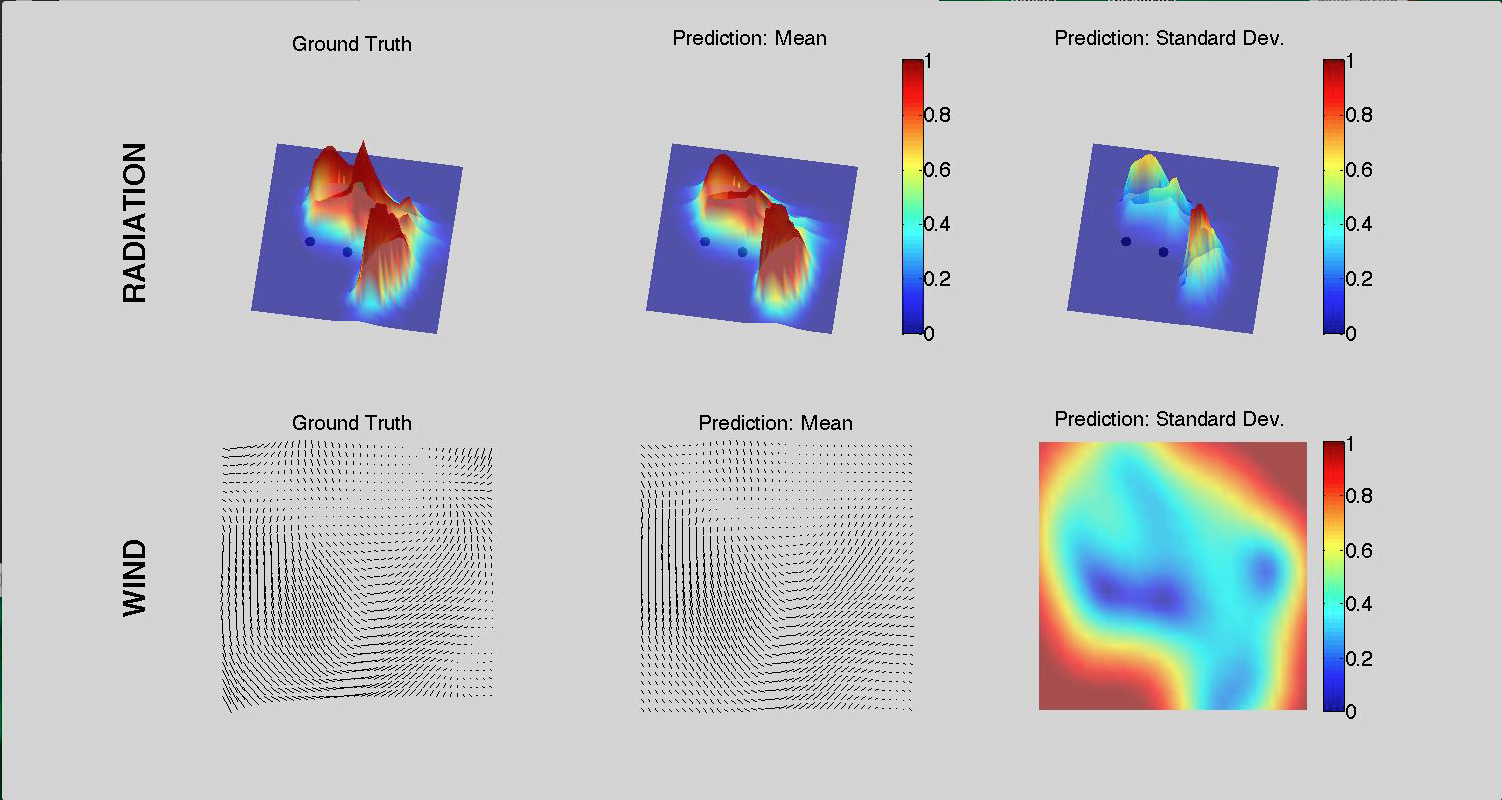
\includegraphics[width=0.45\textwidth]{figures/radiation_ss_calm.png}\\
(a) Slow varying wind conditions\\ \ \\
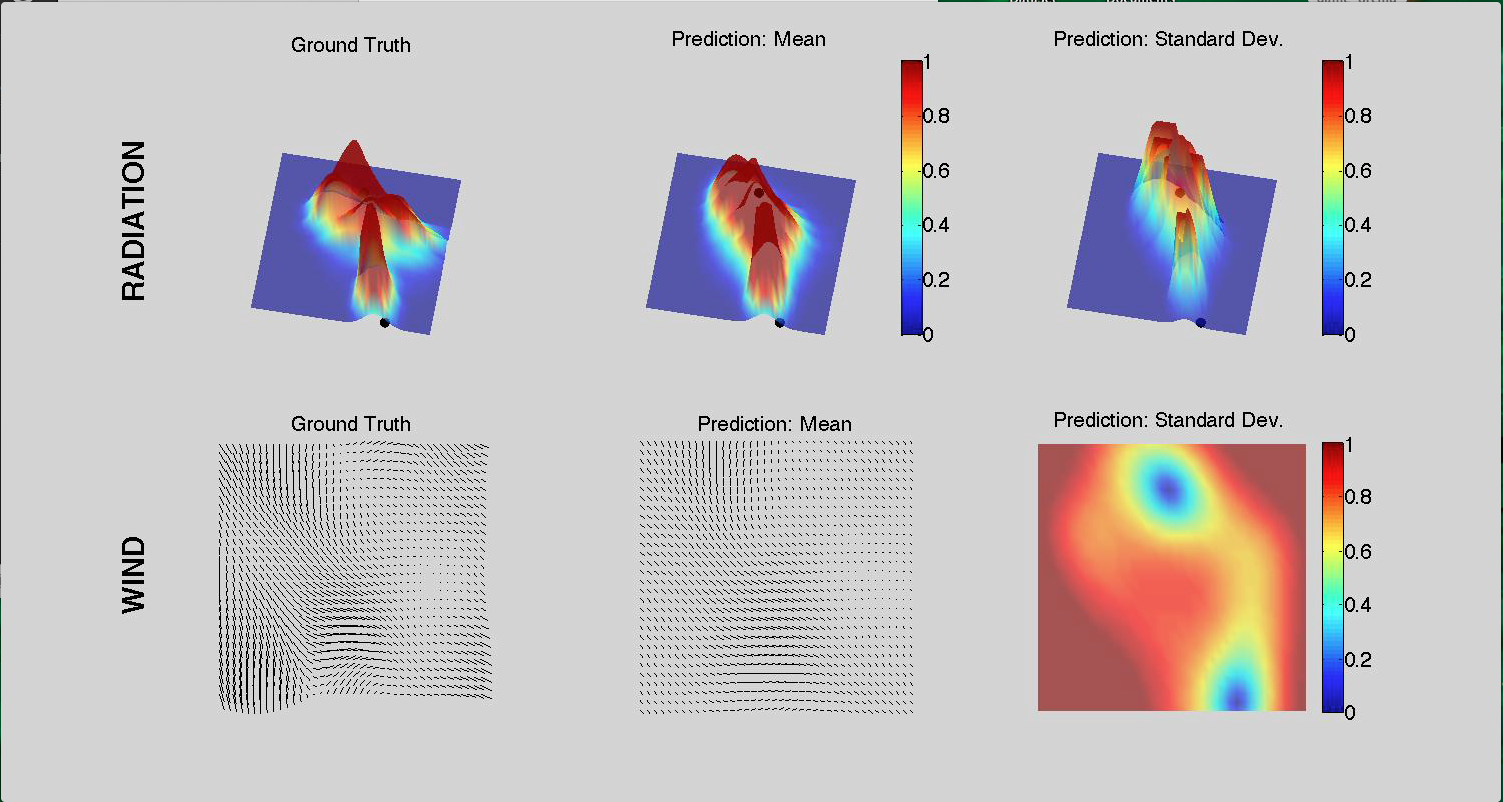
\includegraphics[width=0.45\textwidth]{figures/radiation_ss_gust.png}\\
(b) Gusty wind conditions
\caption{\label{radiation_screen_shots} Radiation and wind simulation ground truth and estimates obtained from monitor agents (black dots).  Left most panes are ground truth, middle panes are estimates and right most panes are estimate uncertainties.  (a) Slow varying wind conditions and (b) gusty wind conditions.}
\end{center}
\end{figure}
